\chapter{Personendetektion}
\label{chap:Personendetektion}



\begin{figure}[H]
	\centering
	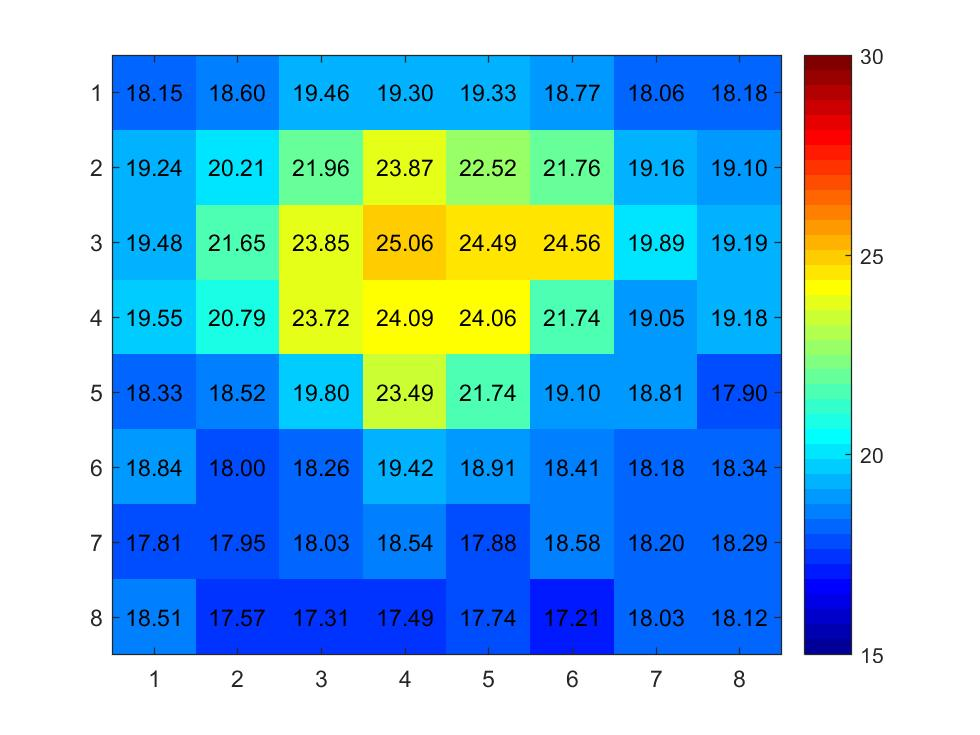
\includegraphics[width=0.5\textwidth]
	{fig/person_175_shirt.jpg}
	\caption[Pixeldarstellung einer Person]{Pxiedarstellung einer Person}
	\label{fig:Pixelbild}
\end{figure}


\section{Datenverarbeitung}

\subsection{Profilierung}





\section{Musterauswertung}



\section{Interpolation}

Die Auflösung von 8x8 Pixel bietet nur begrenzte Aussagekraft. Daher wurde mittels MATLAB mehrere Interpolationsverfahren durchgeführt um die Auflösung der Personenerkennung zu verbessern.





\section{Aufbau neuronales Netzwerk}






\section{Fazit}